\documentclass[a4paper, 12pt, final, garamond]{book}
\usepackage{cours-preambule}

\raggedbottom

\makeatletter
\renewcommand{\@chapapp}{Optique -- chapitre}
\makeatother

\begin{document}
\setcounter{chapter}{3}

\chapter{TD~: dispositifs optiques}

\section{Vergence et grandissement de lentilles accolées}
Soit le système de deux lentilles $\Lc_1$ et $\Lc_2$, de centres optiques
$O_1$ et $O_2$ et de vergences $V_1$ et $V_2$ qui sont \textit{accolées}
(c'est-à-dire de même axe optique et de centres optiques confondus~: dans la
pratique, on veut $|\obar{O_1O_2}| \ll |f_1'|$ et $\ll |f_2'|$ simultanément).

\begin{enumerate}
    \item Montrer qu'il est équivalent à une lentille $\Lc$ de vergence $V = V_1
        + V_2$.
    \item Préciser le grandissement de l'ensemble en fonction du grandissement
        de chaque lentille.
\end{enumerate}

\section{L'œil hypermétrope et sa correction}

Dans cet exercice, on étudie un œil assimilé à une lentille mince convergente
$\Lc$, dont le centre optique $S$ se trouve à une distance constante $d =
\SI{17}{mm}$ de la rétine. Cet œil est hypermétrope et donne d'un objet à
l'infini une image située \SI{1.5}{mm} derrière la rétine lorsqu'il est au repos.

\begin{enumerate}
    \item Déterminer la distance focale de cet œil au repos. On la considèrera
        constante dans la suite du problème, l'œil n'accommodant pas.
    \item L'œil est-il trop ou pas assez convergent ? Corrige-t-on ce défaut en
        ajoutant des verres de lunettes convergents ou divergents ?
    \item L'œil est corrigé par un verre de lunettes, assimilé à une lentille
        mince de centre optique $O$ et
        placé à une distance $d = \SI{12}{mm}$ du centre optique $S$ de l'œil
        réduit. On souhaite que dans ces conditions, l'œil au repos ait une
        vision nette d'un objet situé à l'infini.
        \begin{enumerate}
            \item Rappeler l'endroit où doit se trouver l'image définitive
                donnée par l'œil corrigé.
            \item Quels points caractéristiques du verre et de l'œil doivent
                être confondus afin de corriger la vision de loin ?
            \item Déterminer la distance focale puis la vergence du verre
                correcteur.
            \item Faire un schéma de principe expliquant la correction de l'œil
                par les lunettes.
        \end{enumerate}
\end{enumerate}

\section{Élargissement d'un faisceau laser}
Un laser est un faisceau lumineux cylindrique dont le diamètre est de l'ordre du
millimètre. Comment procéder pour élargir ce faisceau jusqu'à lui donner un
diamètre de quelque centimètres, en utilisant une lentille divergente et une
lentille convergente~?

\section{Étude d'un photocopieur}

\begin{minipage}{0.55\linewidth}
Un photocopieur permet la formation de l'image d'un document sur une surface
photosensible par l'intermédiaire d'un objectif de reproduction. On désire
reproduire un document de format A4 soit en A4 (même format), soit en A3 (format
double en surface) soit en A5 (format moitié en surface). On réalise ces
différents tirages à l'aide d'un objectif en modifiant la position respective
des lentilles à l'intérieur du système. La distance entre le document et le
récepteur photosensible est de \SI{384}{mm} et l'on positionne une première lentille
mince divergente $\Lc_1$ de distance focale image $f'_1 = \SI{-90}{mm}$ à
\SI{180}{mm} du récepteur (figure ci-contre).
\end{minipage}
\begin{minipage}{0.45\linewidth}
    \begin{center}
        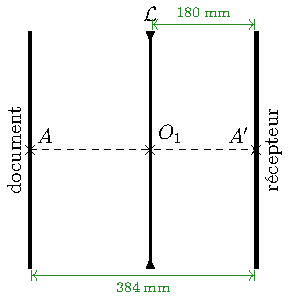
\includegraphics[width=.8\linewidth]{photocopieur-a}
    \end{center}
\end{minipage}

\begin{minipage}{0.55\linewidth}
    \begin{enumerate}
        \item La lentille $\Lc_1$ peut-elle donner une image du document sur le
            récepteur ?
        \item On ajoute une lentille mince $\Lc'$ devant la lentille $\Lc_1$, à
            \SI{180}{mm} du document (voir la figure ci-contre). La lentille
            $\Lc'$ peut-elle être divergente ? Justifier votre réponse.
        \item Calculer la distance focale image $f'$ de cette lentille $\Lc'$
            pour obtenir une image réelle du document sur le récepteur. Pour
            cela, on utilisera deux relations de Descartes.
        \item En déduire le grandissement $\gamma$ de l'association des deux
            lentilles et indiquer quel type de tirage permettra cet objectif :
            transformer du A4 en A3 ou du A4 en A5 ?
    \end{enumerate}
\end{minipage}
\begin{minipage}{0.45\linewidth}
    \begin{center}
        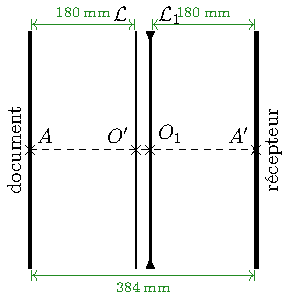
\includegraphics[width=\linewidth]{photocopieur-b}
    \end{center}
\end{minipage}

\section{Le microscope}

Un microscope est schématisé par deux lentilles minces convergentes de même axe
optique~: l'objectif $\Lc_1$ de centre $O_1$ et de distance focale image $f'_1 =
\SI{5}{mm}$, et l'oculaire $\Lc_2$ de centre $O_2$ et de distance focale image
$f'_2 = \SI{25}{mm}$. On note respectivement $F'_1$ et $F_2$ les foyers image de
$\Lc_1$ et objet de $\Lc_2$. On appelle \textit{intervalle optique} et on la
note $\Delta$ la distance $\obar{F'_1F_2} = \SI{25}{cm}$. L'œil de
l'observataire est placé au foyer image $F'_2$ de l'oculaire. On y visualise un
objet étendu transverse $AB$ avec $A$ sur l'axe optique.

\begin{enumerate}
    \item Où doit se situer $A$ pour que l'œil n'ait pas à accommoder~? Répondre
        en donnant l'expression et la valeur numérique de $\obar{F_1A}$.
    \item On se place dans les conditions de la question précédente. Représenter
        le trajet de 2 rayons issus de $B$ sur une figure horizontale respectant
        le fait que $f'_1 < f'_2 < \Delta$.
    \item Soient $\alpha'$ l'angle algébrique sous lequel l'œil voit l'image
        finale de $AB$ par le microscope, et $\alpha$ l'angle algébrique sous
        lequel il apercevrait l'objet sans microscope et à la distance $\Delta$.
        Calculer le grossissement, et interpréter son signe.
\end{enumerate}

\section{Lunettes astronomiques de Kepler et Galilée}

\subsection{Kepler}

On construit une lunette astronomique de Kepler par un objectif $\Lc_1$ de
diamètre $D = \SI{30}{mm}$, de centre $O_1$ et de vergence $V_1 =
\SI{3.125}{\delta}$, et d'un oculaire $\Lc_2$ de centre $O_2$ et de vergence
$V_2 = \SI{25}{\delta}$.

\begin{enumerate}
    \item Calculer les distances focales images $f'_1$ et $f'_2$ de l'objectif
        et de l'oculaire respectivement.
    \item Définir le caractère afocal d'une lunette et son intérêt pour un
        œil emmétrope.
    \item Calculer alors l'encombrement $\obar{O_1O_2}$ de la lunette.
    \item Faire un schéma à l'échelle avec comme rayons incident~:
        \begin{itemize}
            \item Un rayon passant par $O_1$ venant d'en haut~;
            \item Deux rayons proches, parallèles entre eux et au premier rayon.
        \end{itemize}
        On prendra soin de~:
        \begin{enumerate}
            \item placer l'image intermédiaire donnée par l'objectif~;
            \item puis l'image finale donnée par l'oculaire~;
            \item tracer le cheminement du pinceau lumineux entre les deux
                rayons proches (on hachurera la zone qu'ils délimitent).
        \end{enumerate}
    \item Calculer le grossissement de la lunette.
    \item Rappeler la définition du cercle oculaire et son intérêt.
    \item Déterminer sa position $\obar{O_2C'_K}$.
    \item Donner sa taille (diamètre $D'_K$).
\end{enumerate}

\subsection{Galilée}

On obtient une lunette de Galilée en remplaçant l'oculaire convergent par un
oculaire divergent. Dans cet exercice, la valeur de la vergence est la même que
précédemment en valeur absolue. On nomme cette lentille $\Lc_3$, son centre sera
noté $O_3$. La lunette astronomique reste afocale.

\begin{enumerate}
    \item Expliquer que la vergence de l'oculaire sera $V_3 = \SI{-25}{\delta}$.
    \item Calculer le nouvel encombrement $\obar{O_1O_3}$.
    \item Tracer, toujours à l'échelle, le même schéma que précédemment avec
        cette nouvelle situation.
    \item Déterminer la position $\obar{O_3C'_G}$ du cercle oculaire.
    \item Donner sa taille (diamètre $D'_G$).
    \item Quels sont les avantages et inconvénients de ces 2 lunettes
        astronomiques~?
\end{enumerate}

\end{document}
